\section{Introduzione}
\begin{frame}{Contesto}

L’inquinamento atmosferico è uno dei principali problemi che interessano le aree urbanizzate.
\vspace{0.3cm}
\begin{itemize}
 \item Può portare a problemi di salute causati dall’esposizione a lungo termine a sostanze nocive (PM, \ce{NO2}, \ce{CO2}, \ce{O3})\vspace{0.3cm}
 \item Il monitoraggio è essenziale per la tutela della salute pubblica\vspace{0.1cm}
 \begin{enumerate}
 \item Con reti regionali di rilevamento fisse, gestite da ARPA (DLgs. n.155 del 13/08/2010)\vspace{0.1cm}
 \item Con nuove reti di sensori \textit{low cost} ad alta portabilità per l'acquisizione di misure aggiuntive, anche a minor precisione (es. \textbf{AirQino})
\end{enumerate}
\end{itemize}

\end{frame}

\begin{frame}{La piattaforma AirQino (1/3)}
\begin{columns}

\begin{column}{0.45\textwidth}

\begin{itemize}
  \item Monitoraggio ambientale ad alta precisione
  \item Configurabile ed estendibile
  \item Dati in tempo reale
\end{itemize}\vspace{0.1cm}

\begin{figure}[H]
\centering
\captionsetup{justification=centering}
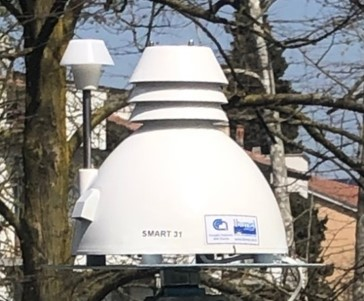
\includegraphics[width=.6\textwidth]{images/airqino_stazione}
\caption{Una centralina AirQino}
\end{figure}

\end{column}

\begin{column}{0.65\textwidth}

\begin{center}
\alert{https://airqino.magentalab.it}
\vspace{-0.3cm}
\begin{figure}[H]
\centering
\captionsetup{justification=centering}
\includegraphics[width=\textwidth]{images/airqino_web_n}
\caption{Pagina web AirQino}
\end{figure}
\end{center}

\end{column}

\end{columns}
\end{frame}

\begin{frame}[t]{La piattaforma AirQino (2/3) – Architettura}
\begin{center}

\begin{figure}[H]
\centering
\captionsetup{justification=centering}
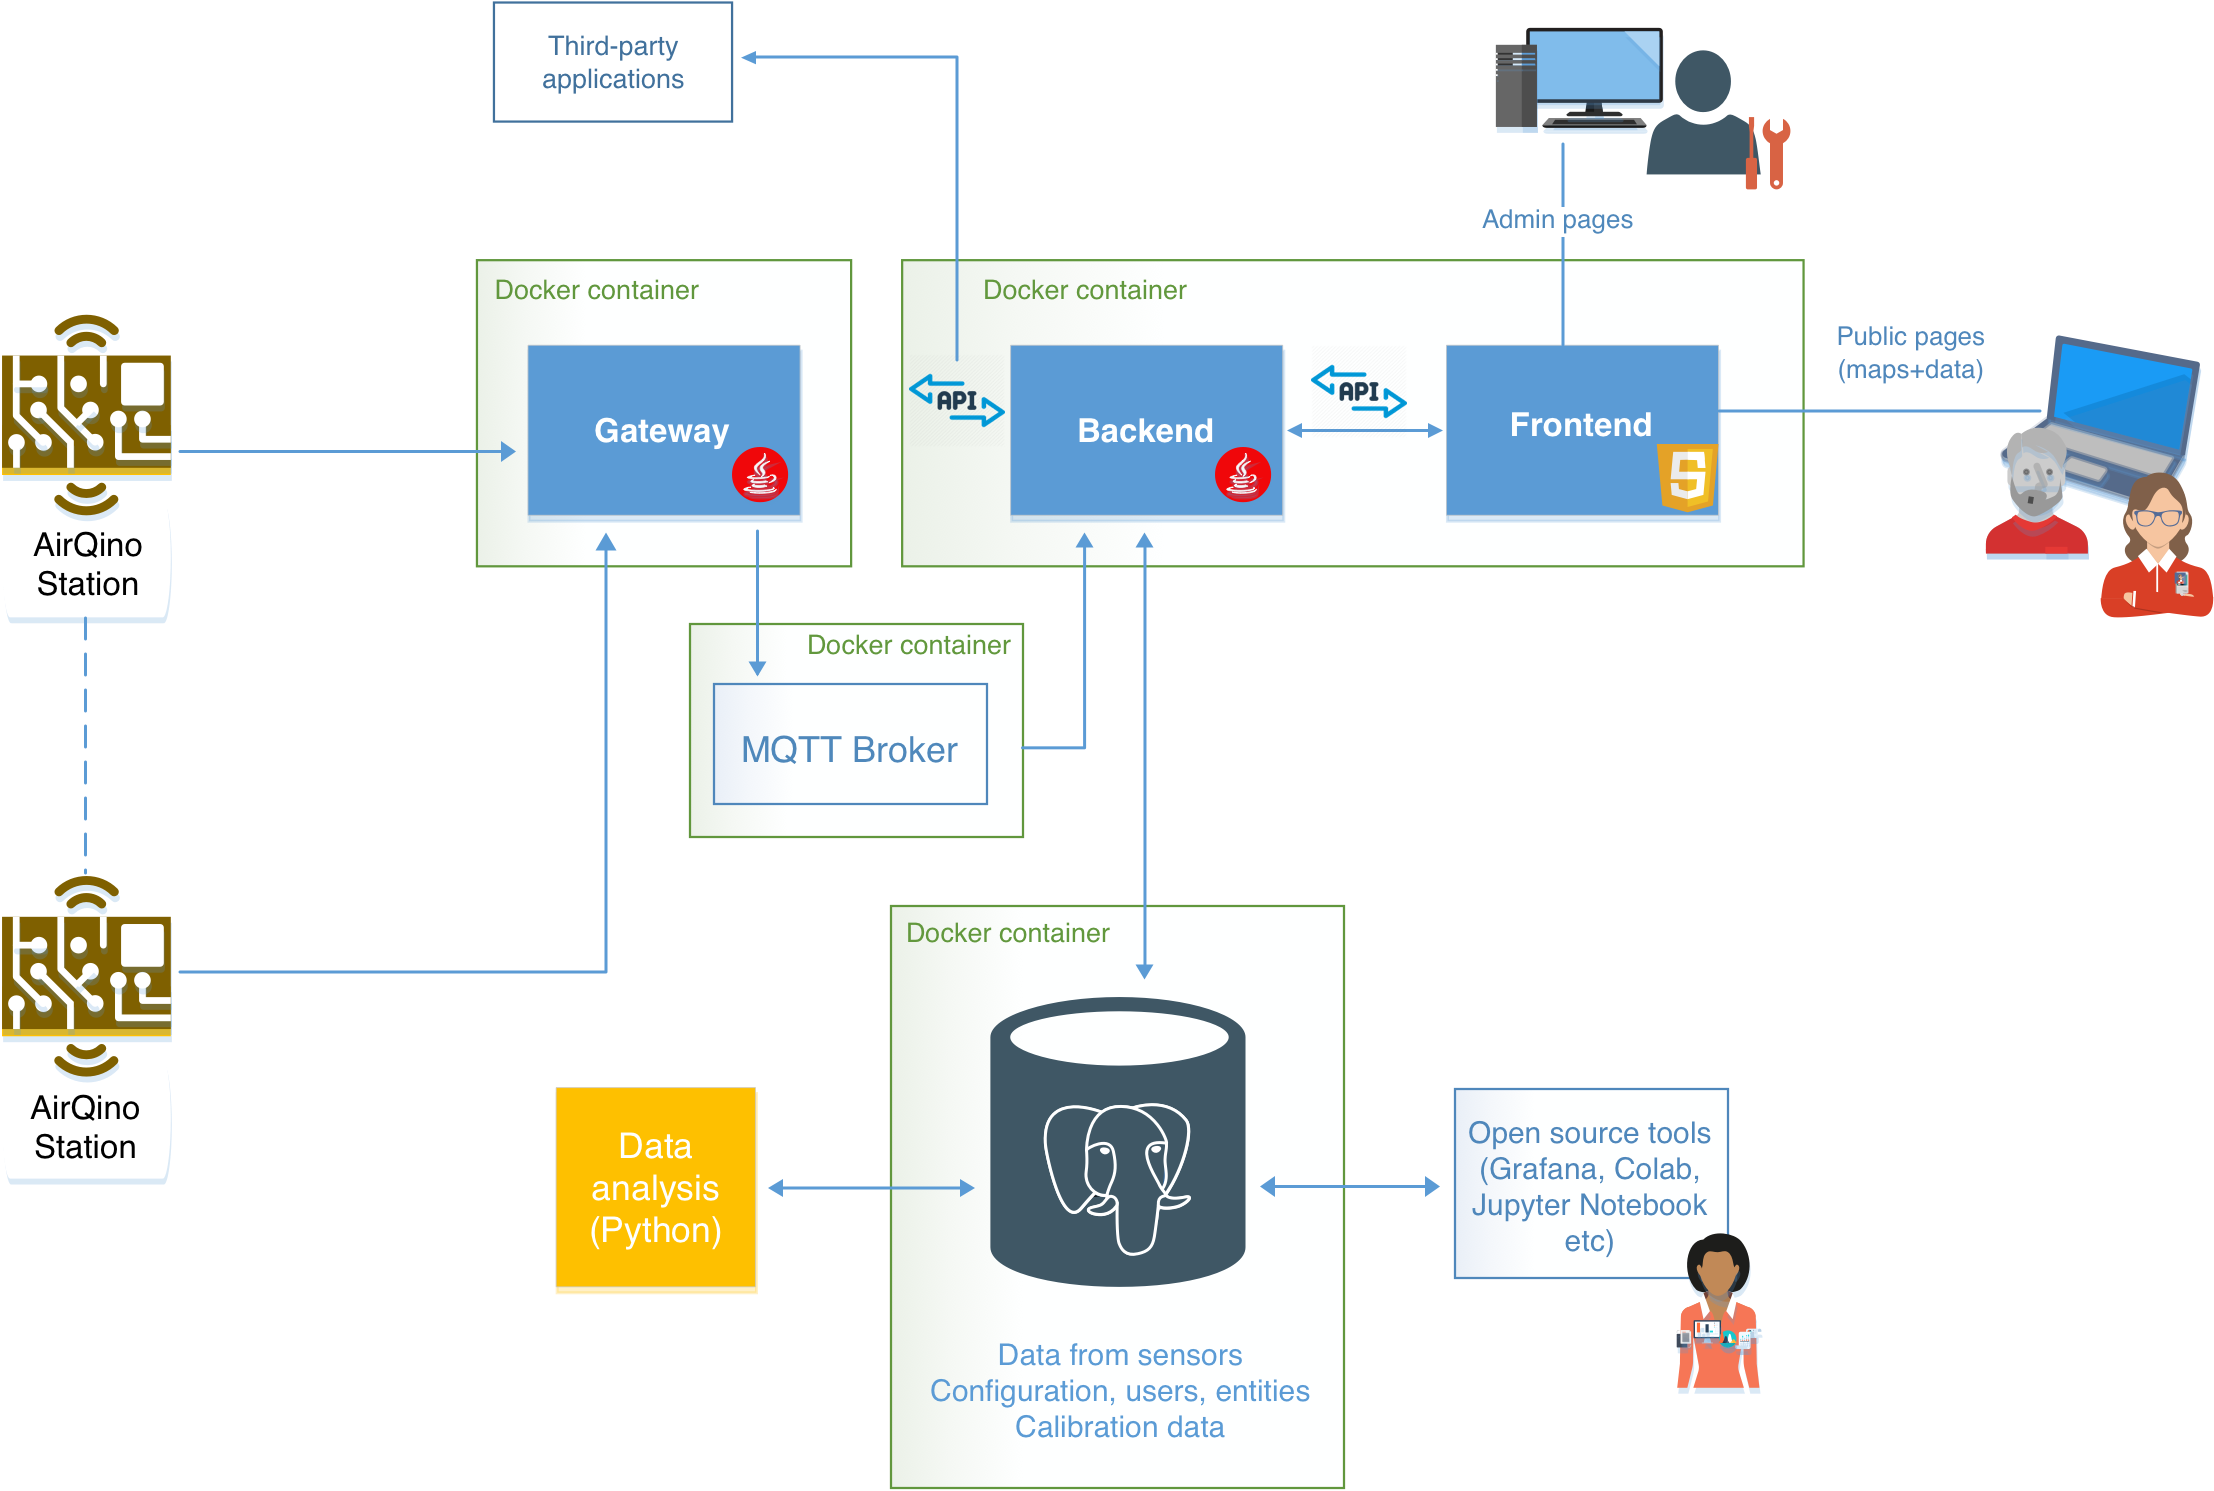
\includegraphics[width=.8\textwidth]{images/airqino_arch.png}
\caption{Architettura della piattaforma}
\end{figure}

\end{center}
\end{frame}

\begin{frame}[t]{La piattaforma AirQino (3/3) – Sensori}
\begin{columns}

\begin{column}{0.5\textwidth}
\begin{center}

\begin{block}{MiCS-2714 per \ce{NO2}}
\begin{figure}[H]
    \centering
    \subfloat[\centering Sensore]{{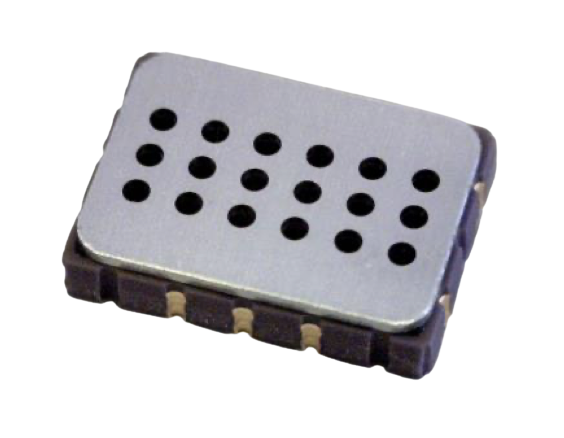
\includegraphics[width=2.4cm]{images/mics1-removebg-preview} }}
    \subfloat[\centering Circuito]{{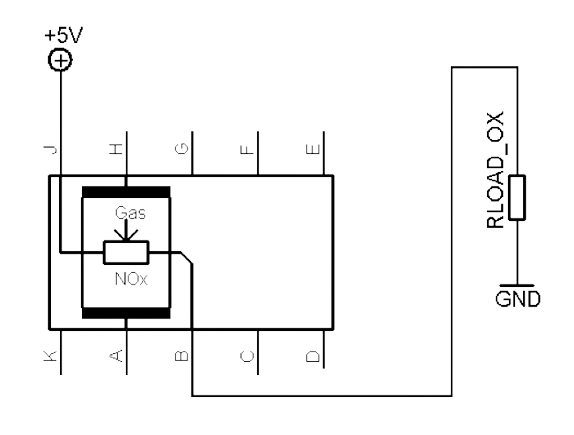
\includegraphics[width=2.4cm]{images/mics2-removebg-preview} }}
\end{figure}
\vspace{0.1cm}
\begin{itemize}
  \item Di tipo MOS, basato su \textit{ossidoriduzione}
  \item Uscita in \textit{counts}
  \item Costo: meno di 5€
\end{itemize}
\vspace{0.1cm}

\end{block}

\end{center}
\end{column}

\begin{column}{0.5\textwidth}
\begin{center}
\begin{block}{SDS011 per \ce{PM_{2.5}} e \ce{PM_{10}}}
\begin{figure}[H]
    \centering
    \subfloat[\centering Sensore]{{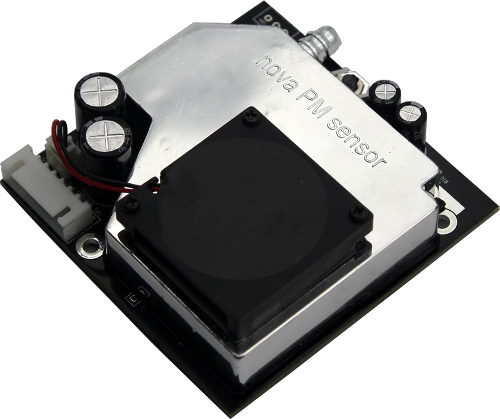
\includegraphics[width=2cm]{images/sds1} }}
    \subfloat[\centering Componenti]{{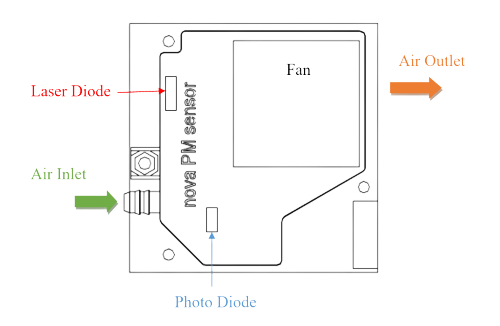
\includegraphics[width=2.7cm]{images/sds2_rmbg} }}
\end{figure}
\vspace{0.1cm}
\begin{itemize}
  \item Basato su \textit{scattering}
  \item Uscita in $\mathrm{\si{\micro}g/m^3}$
  \item Costo: 25€ circa
\end{itemize}
\vspace{0.1cm}

\end{block}
\end{center}
\end{column}

\end{columns}
\end{frame}

\begin{frame}{Obiettivi}
\begin{itemize}
  \item Sviluppi tecnologici alla piattaforma
  \begin{enumerate}
    \item Miglioramento dell'\textbf{affidabilità} dei dati provenienti dai sensori
    \item Riduzione dei \textbf{tempi di risposta} dal database
  \end{enumerate}\vspace{0.3cm}
  \item Studio e confronto tra diverse tecniche volte a migliorare l’accuratezza del processo di \textbf{calibrazione} dei sensori (sia \ce{NO2} che PM)\vspace{0.3cm}
  \item Sviluppo di un’\textbf{interfaccia web} per facilitare la calibrazione \textit{massiva} di centraline
\end{itemize}
\end{frame}


\section{Sviluppi tecnologici}
\begin{frame}{Sviluppi – Replica del database (1/2)}
\begin{block}{Replica}
Tutti i dati del database vengono copiati e distribuiti su un altro spazio fisico. 

La nuova istanza agisce come nodo secondario, alleggerendo il carico dal database primario. 

\vspace{0.4cm}
\textbf{Vantaggi:}\vspace{0.1cm}
\begin{itemize}
  \item Maggiore \textbf{affidabilità}
  \item Miglioramento delle \textbf{prestazioni}
  \item Maggiore \textbf{sicurezza} dei dati
\end{itemize}\vspace{0.1cm}
\end{block}

\end{frame}

\begin{frame}{Sviluppi – Replica del database (2/2)}

\begin{columns}

\begin{column}{0.45\textwidth}
\begin{block}{Streaming replication}
Funzionalità che consente di replicare i dati in tempo reale da una istanza di database Postgres a un’altra

\begin{itemize}
  \item Replica di sola lettura
  \item Basata su \textbf{WAL} (\textit{Write Ahead Log})
  \item Automazione con Docker\vspace{0.1cm}
\end{itemize}
\end{block}
\end{column}

\begin{column}{0.55\textwidth}
\begin{figure}[H]
\centering
\captionsetup{justification=centering}
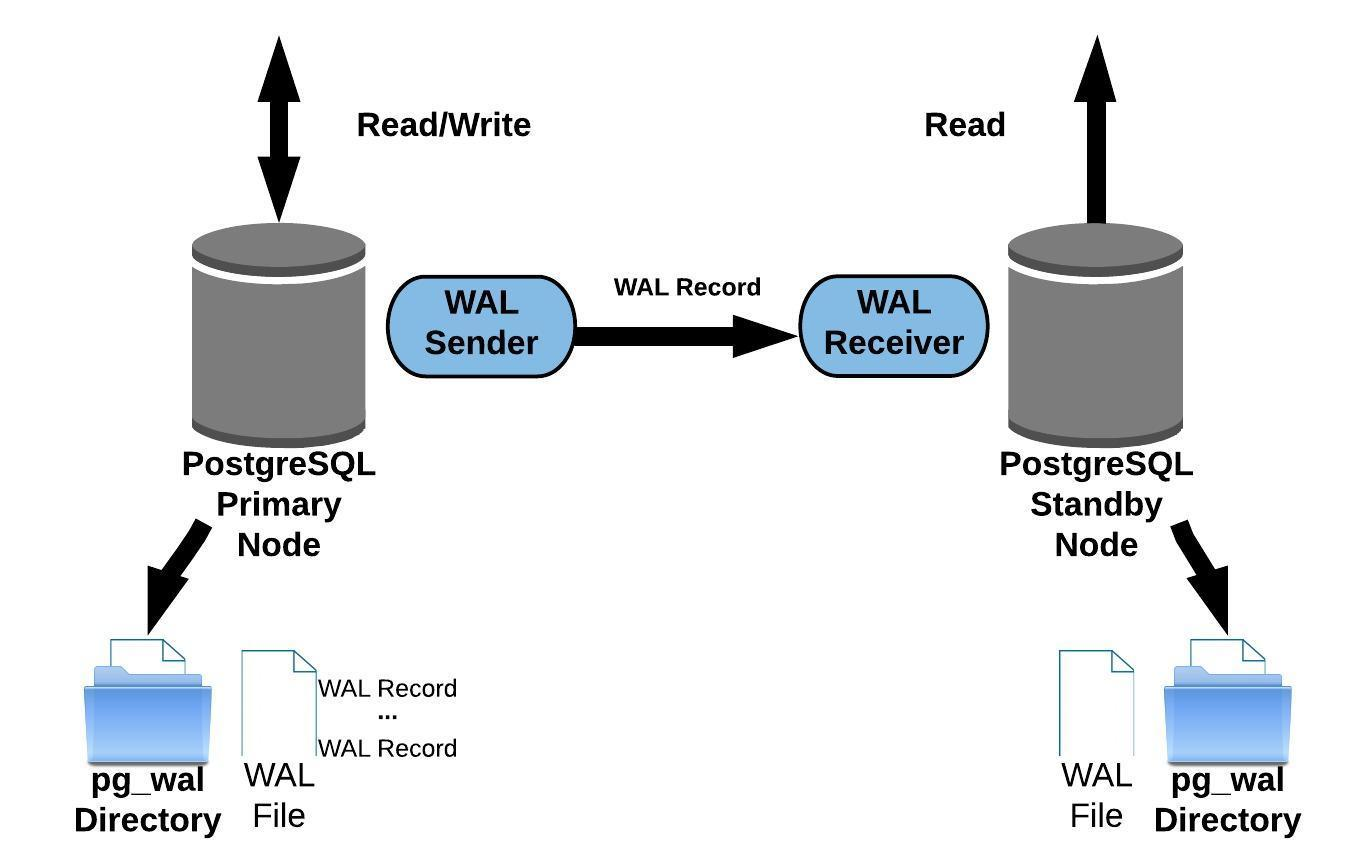
\includegraphics[width=\textwidth]{images/streaming_replication}
\caption{Streaming replication}
\end{figure}
\end{column}

\end{columns}

\end{frame}


\begin{frame}{Sviluppi – Ottimizzazione di query temporali (1/2)}

\begin{columns}

\begin{column}{0.45\textwidth}
\begin{block}{Continuous aggregates}
Funzionalità di \textbf{Timescale} per aggregare dati in tempo reale in maniera incrementale

\begin{itemize}
  \item Miglioramento delle \textbf{performance}
  \item Aggiornamento \textbf{automatico} in background
  \item Risparmio di \textbf{spazio}\vspace{0.1cm}
\end{itemize}
\end{block}
\end{column}

\begin{column}{0.55\textwidth}
\begin{figure}[H]
\centering
\captionsetup{justification=centering}
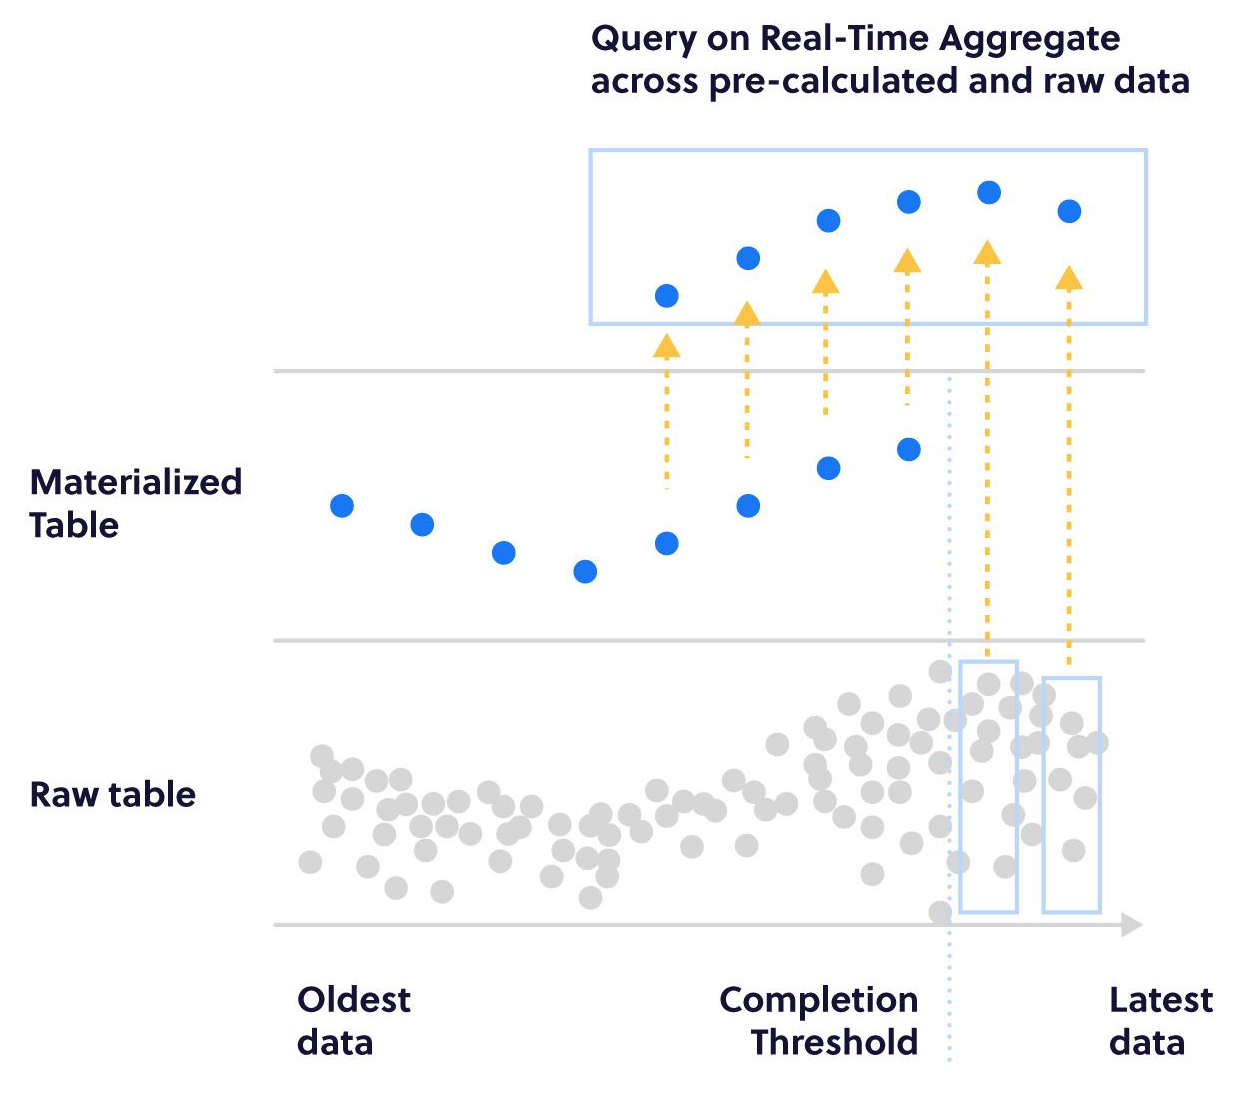
\includegraphics[width=\textwidth]{images/continuous_aggregates_r}
\caption{Continuous aggregates}
\end{figure}
\end{column}

\end{columns}

\end{frame}

\begin{frame}{Sviluppi – Ottimizzazione di query temporali (2/2)}
Tempi di risposta della query per estrarre la media oraria di \ce{NO2} dell'ultima settimana da tutte le centraline \textbf{AirQino}:

\begin{columns}
\begin{column}{0.55\textwidth}
\begin{figure}[H]
\centering
\captionsetup{justification=centering}
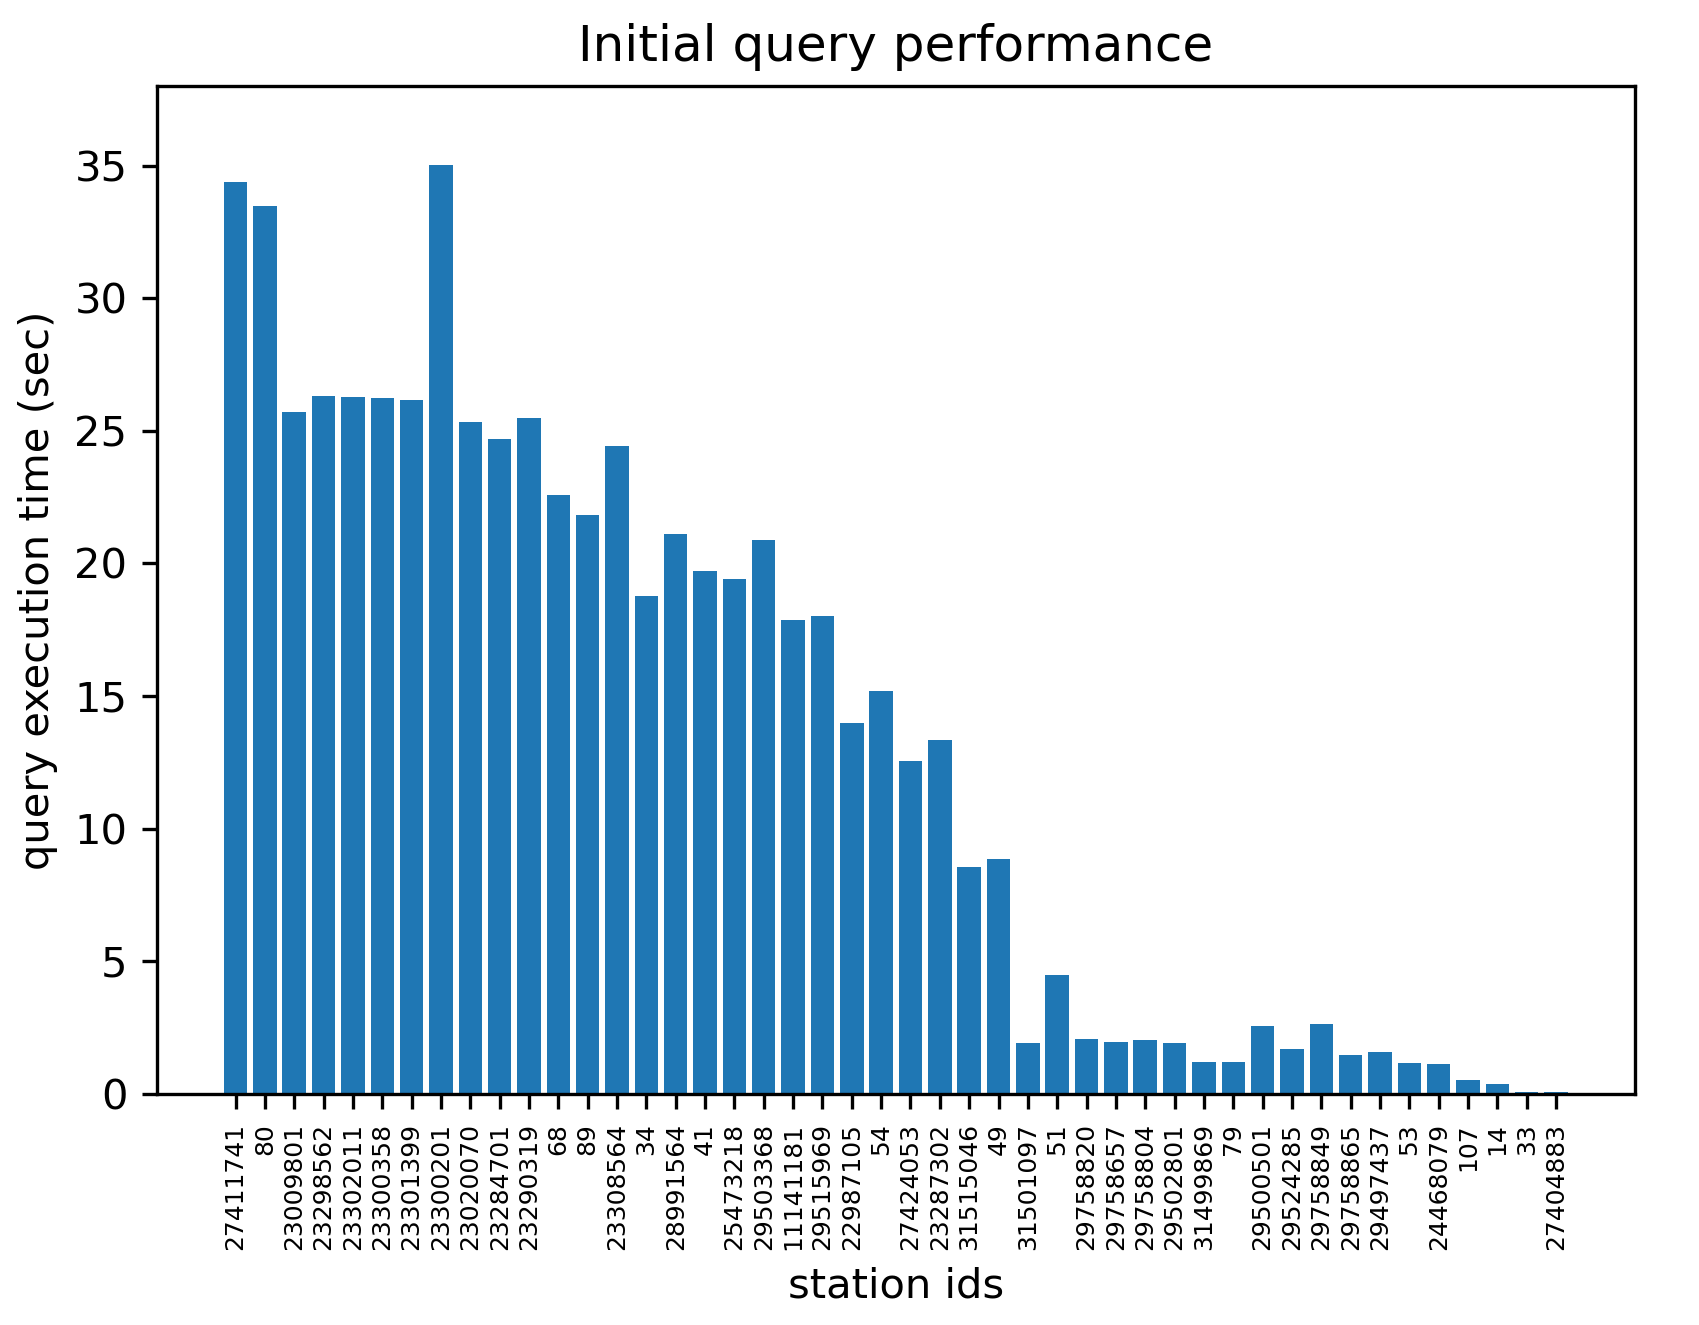
\includegraphics[width=\textwidth]{images/query_prima}
\caption{Prima dell'ottimizzazione}
\end{figure}
\end{column}

\begin{column}{0.55\textwidth}
\begin{figure}[H]
\centering
\captionsetup{justification=centering}
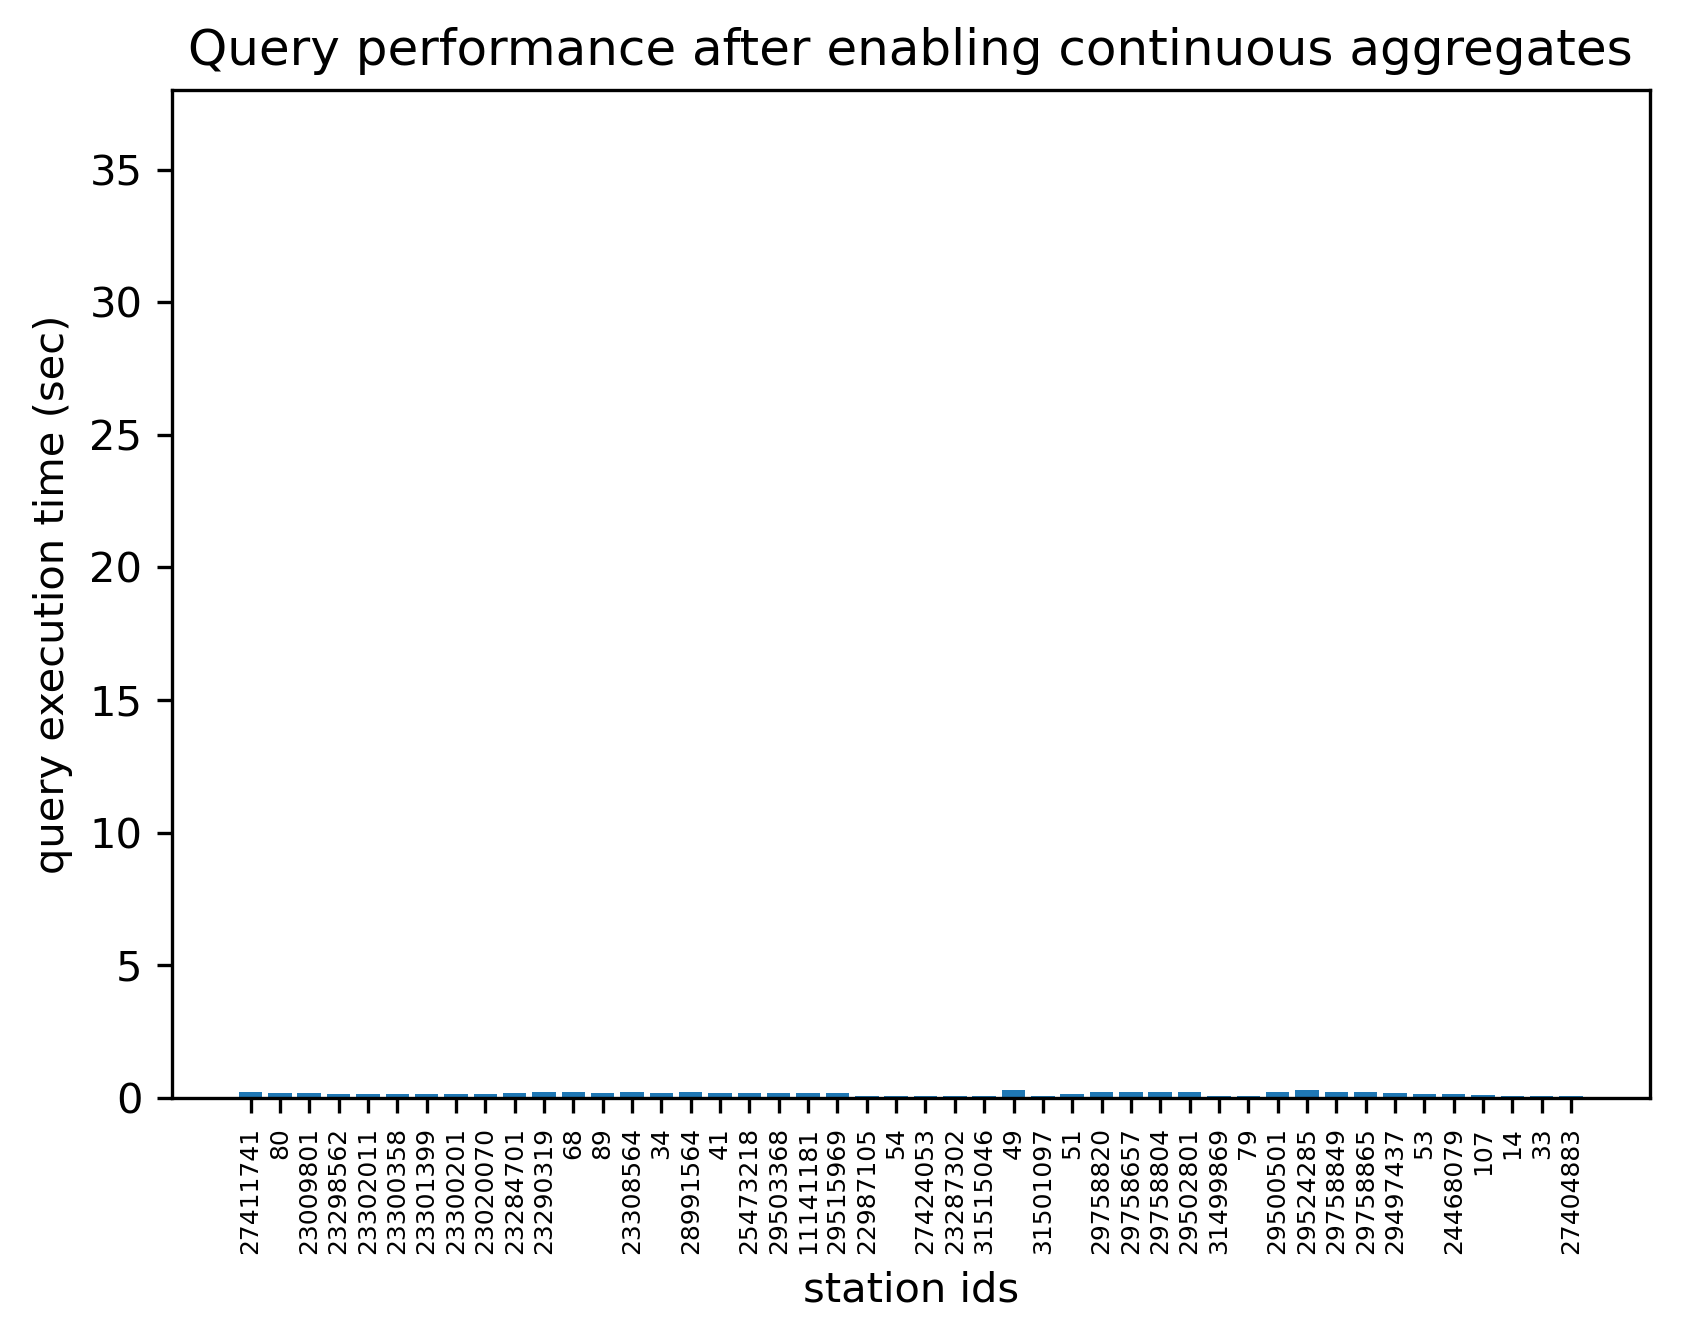
\includegraphics[width=\textwidth]{images/query_dopo}
\caption{Dopo l'ottimizzazione}
\end{figure}
\end{column}
\end{columns}

\end{frame}


\section{Calibrazione}

\begin{frame}{Calibrazione (1/4) – Procedura}
comparazione verso sensori di riferimento
confronto delle concentrazioni rilevate dalle stazioni di riferimento ARPAT
\begin{block}{Procedura per ogni sensore (\ce{NO2}, \ce{PM_{2.5}}, \ce{PM10})}
\begin{enumerate}
  \item Preprocessamento e creazione di un \textbf{dataset} (dati della centralina AirQino SMART16 e di riferimento ARPAT)
  \item \textbf{Allineamento} temporale e ricampionamento
  \item \textbf{Scatterplot} del segnale di riferimento e del segnale del sensore
  \item Analisi dei \textbf{residui}
  \item Applicazione di tredici diversi modelli di \alert{regressione}
  \begin{itemize}
    \item Su tutto il dataset
    \item Con cadenza mensile
  \end{itemize}
  \item Valutazione della \textbf{performance} in termini di $R^2$ e $RMSE$
  \item \textbf{Validazione} del modello più performante\vspace{0.1cm}
\end{enumerate}
\end{block}

\end{frame}

\begin{frame}{Calibrazione (2/4)  – Risultati}
\begin{columns}

\begin{column}{0.55\textwidth}

\begin{center}
\begin{figure}[H]
\centering
\captionsetup{justification=centering}
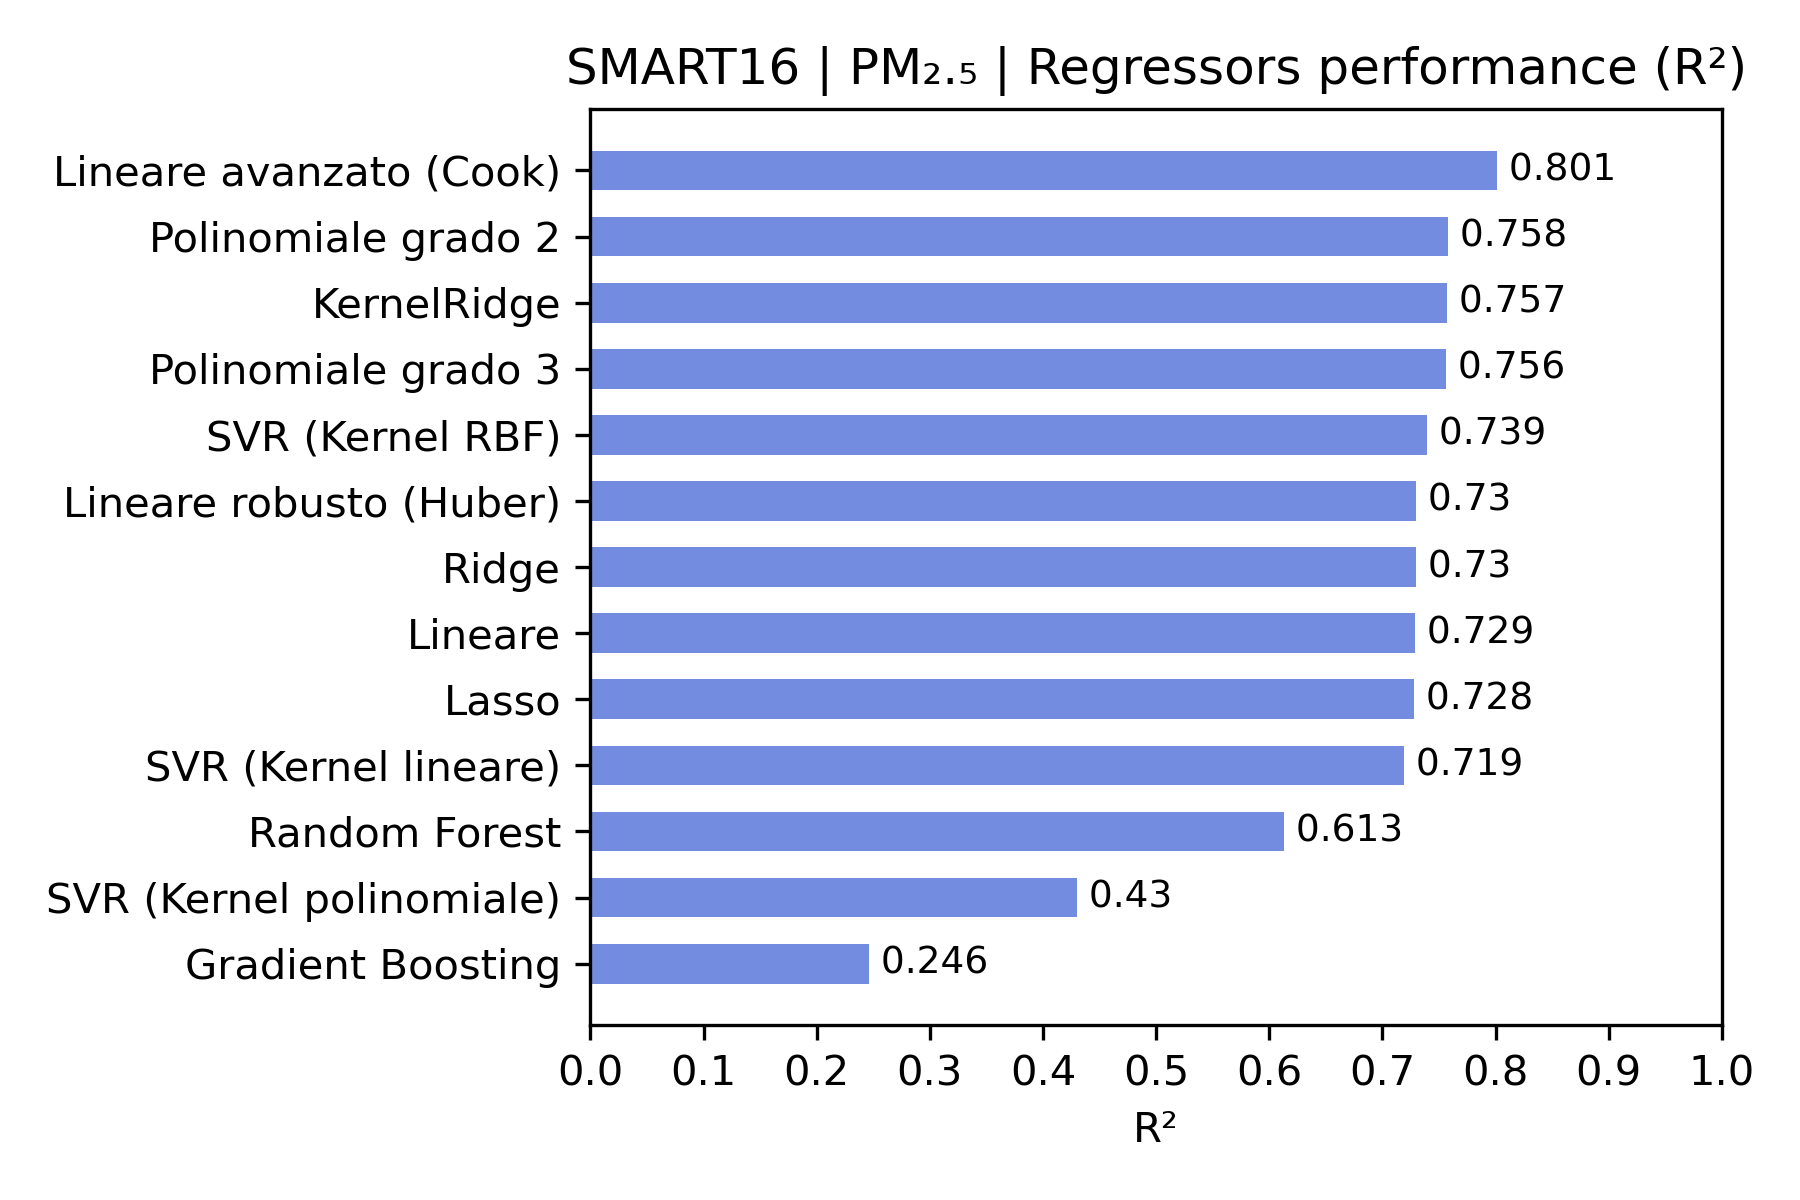
\includegraphics[width=\textwidth]{images/hist_pm2.5_1.png}
\caption{Risultati \ce{PM_{2.5}} ($R^2$)}
\end{figure}
\end{center}

\end{column}
\begin{column}{0.55\textwidth}

\begin{center}
\begin{figure}[H]
\centering
\captionsetup{justification=centering}
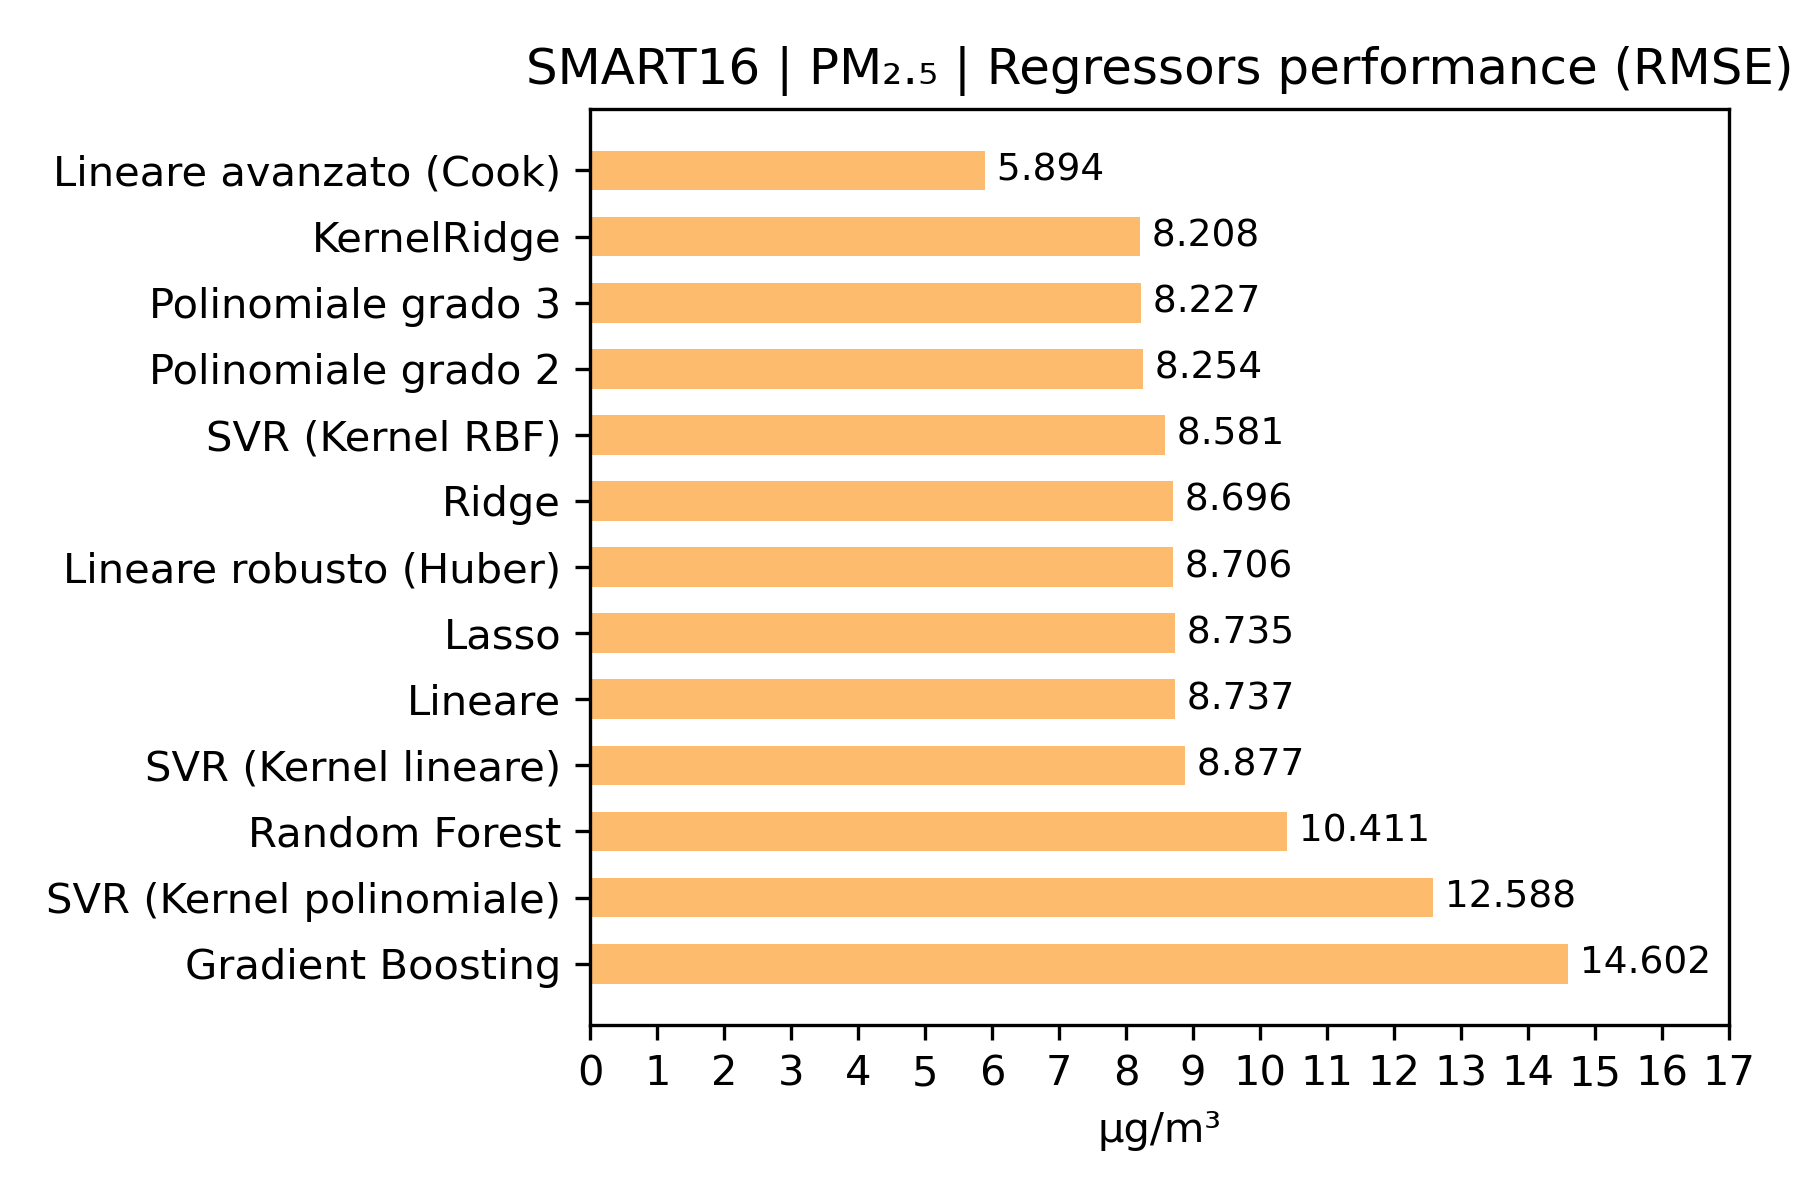
\includegraphics[width=\textwidth]{images/hist_pm2.5_2.png}
\caption{Risultati \ce{PM_{10}} ($RMSE$)}
\end{figure}
\end{center}

\end{column}
  
\end{columns}

\end{frame}

\begin{frame}{Calibrazione (3/4) – Modello più performante}

\begin{columns}
\hspace{0.3cm}\begin{column}{0.45\textwidth}

\begin{block}{Regressione lineare avanzata}
Con rimozione dei valori anomali (\textit{outlier}) in base a determinate metriche.\vspace{0.2cm}

\textbf{Distanza di Cook\footnotemark:}
$$D_{i}=\frac{\sum_{j=1}^{n}\left(\hat{y}_{j}-\hat{y}_{j(i)}\right)^{2}}{p  * MSE^{2}}$$

\textbf{Soglia di cut-off\,\footnotemark}:
$D_{i}>\frac{4}{n}$

\vspace{0.1cm}
\end{block}
\end{column}

\hspace{0.1cm}\begin{column}{0.55\textwidth}

\begin{center}
\begin{figure}[H]
\centering
\captionsetup{justification=centering}
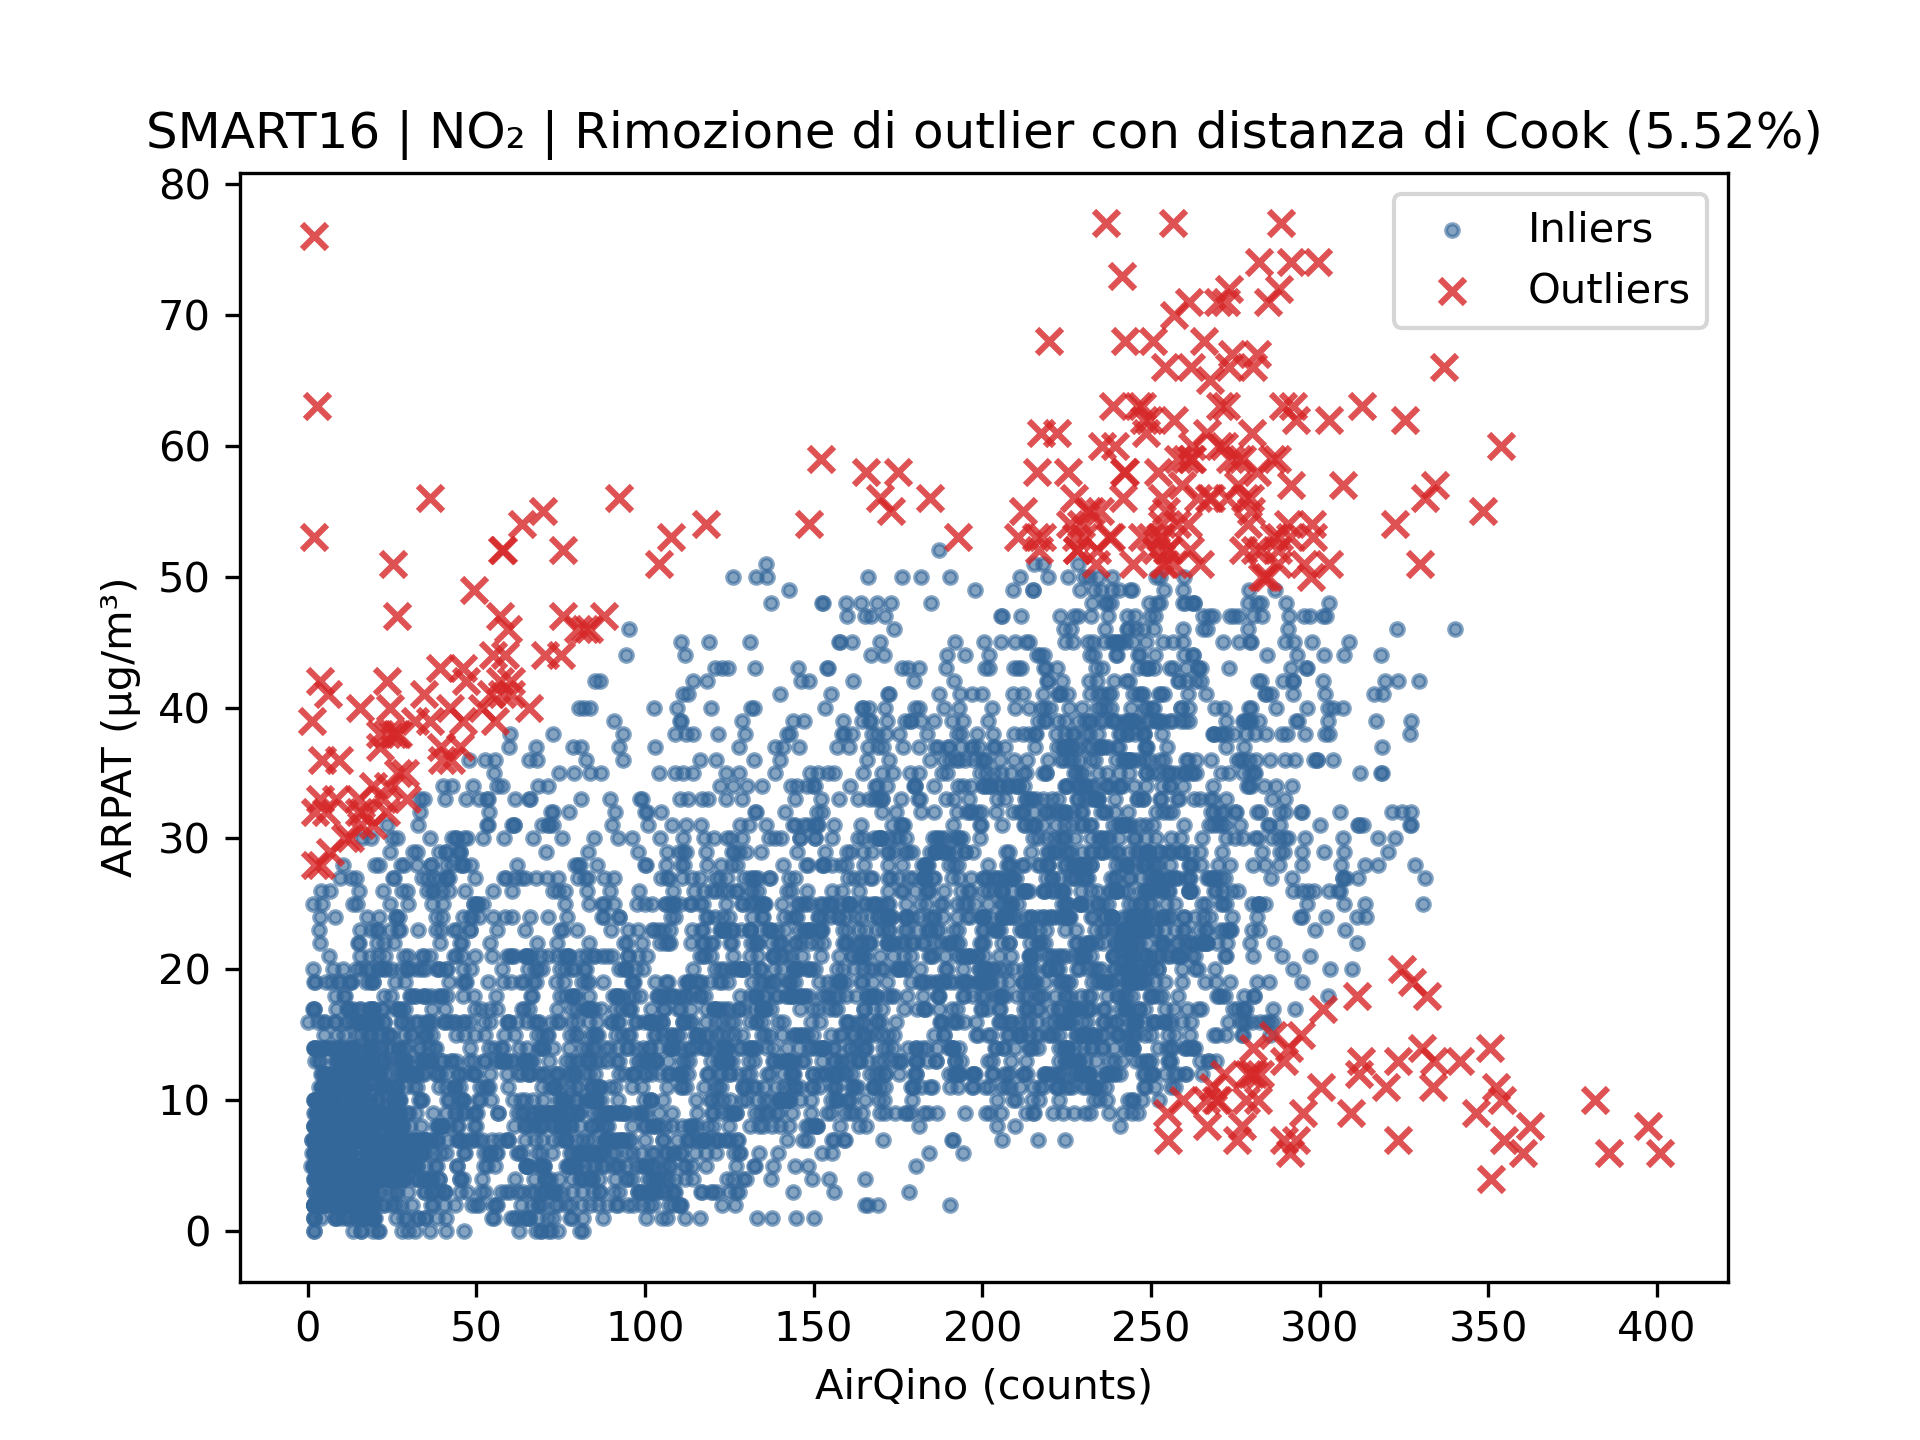
\includegraphics[width=\textwidth]{images/cook_no2.png}
\caption{Rilevamento di \textit{outlier} (in rosso) tramite distanza di Cook}
\end{figure}
\end{center}

\end{column}

\let\oldfootnotesize\footnotesize
\renewcommand*{\footnotesize}{\oldfootnotesize\tiny}
\addtocounter{footnote}{-1}\footnotetext{\fullcite{cook_def}}
\addtocounter{footnote}{1}\footnotetext{\fullcite{applied_regression}\vspace{0.05cm}}

\end{columns}

\end{frame}

\begin{frame}{Calibrazione (4/4) – Validazione}
\begin{center}
\begin{figure}[H]
\centering
\captionsetup{justification=centering}
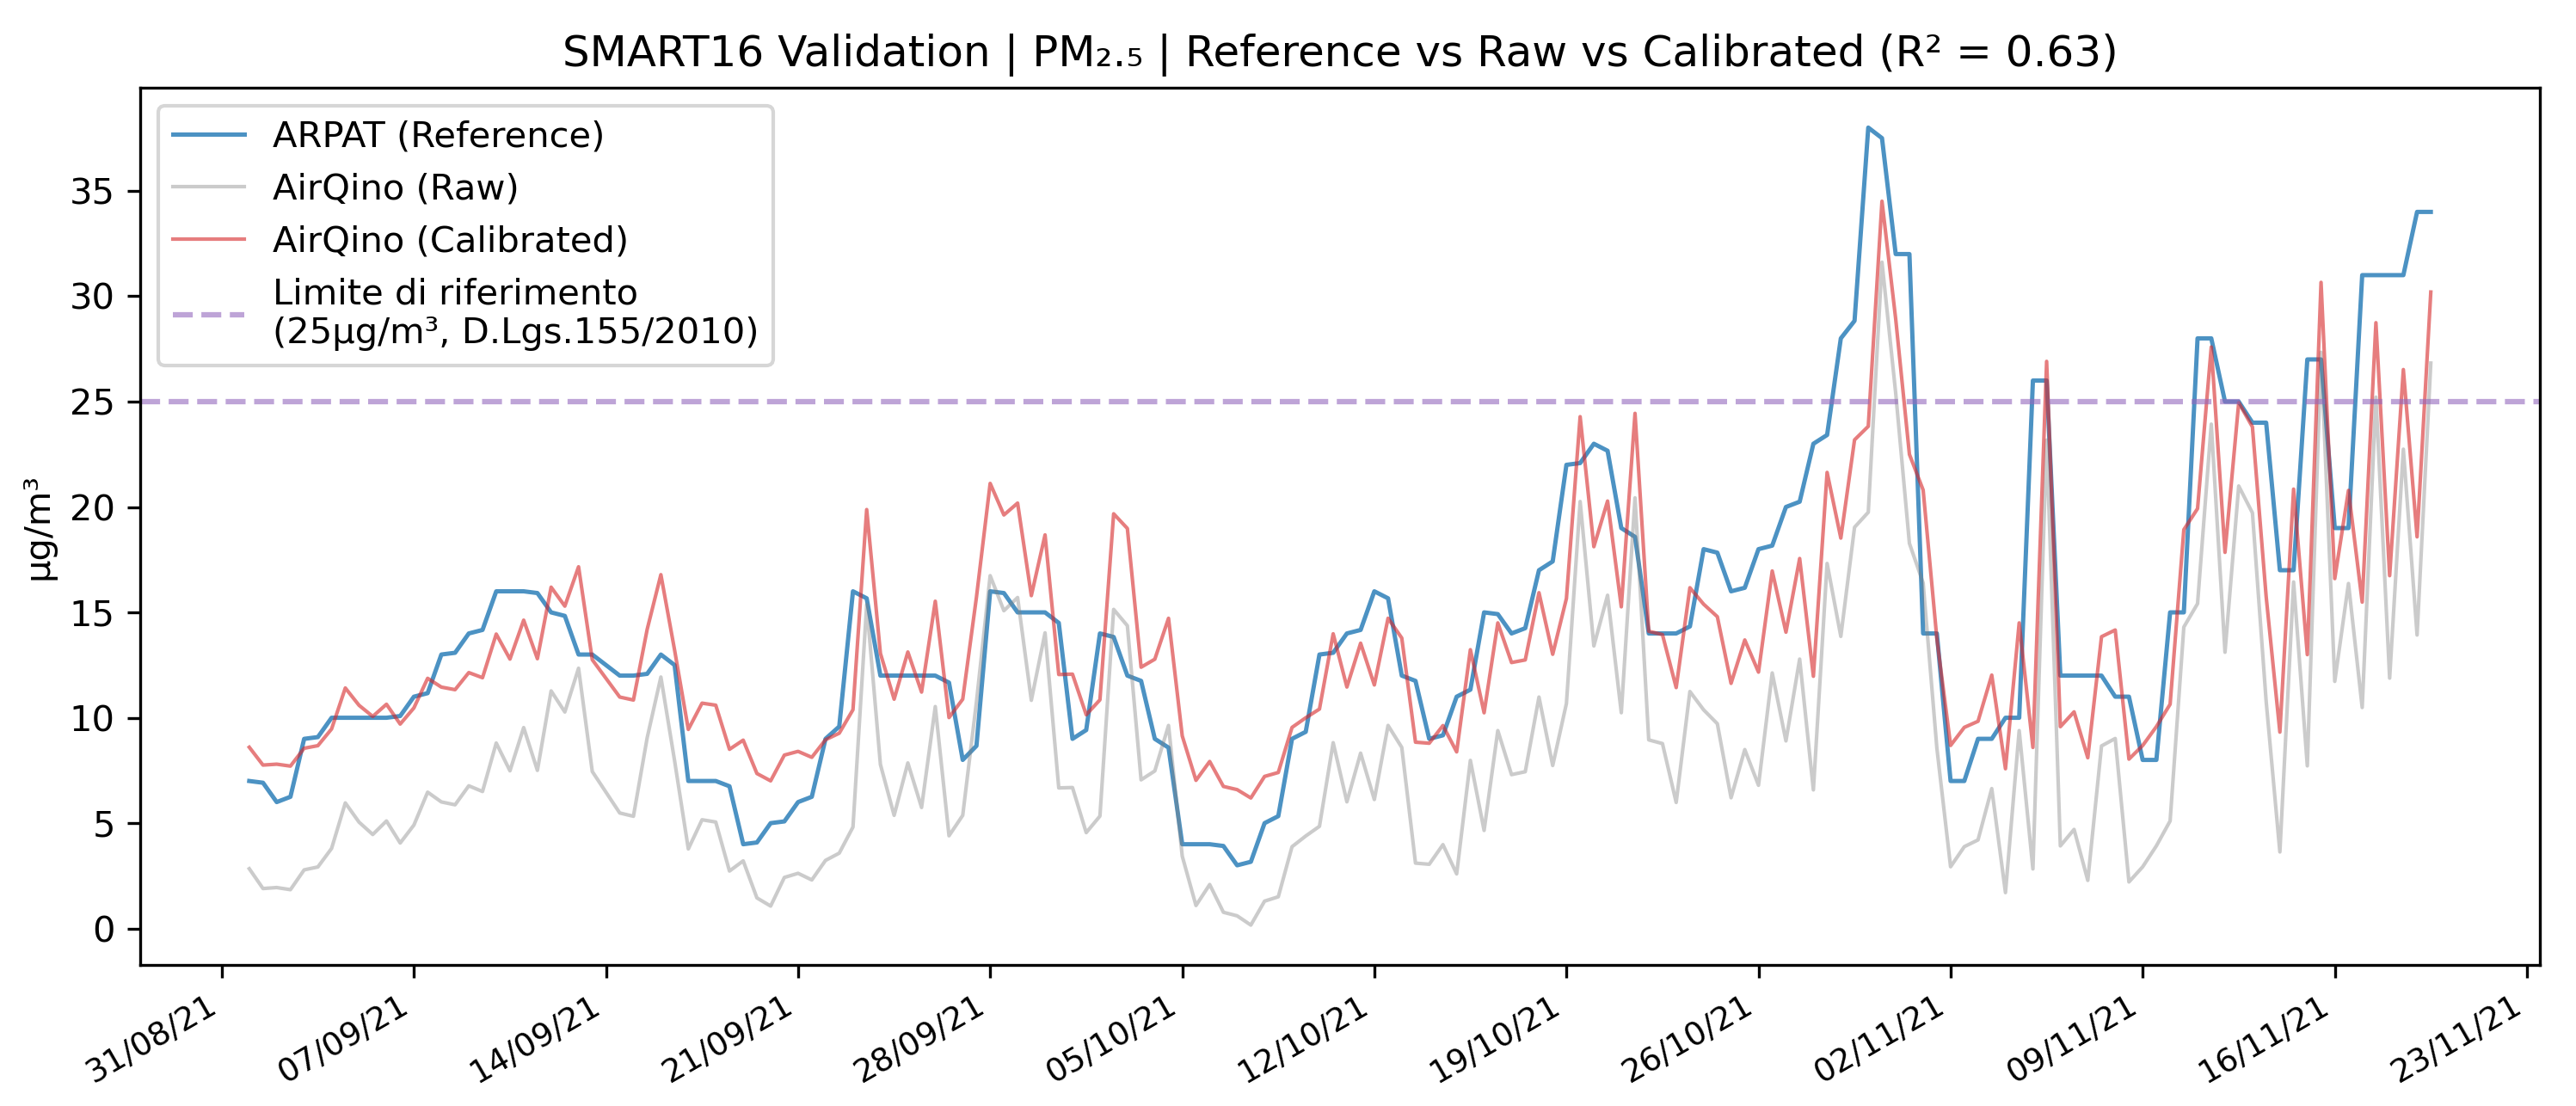
\includegraphics[width=\textwidth]{images/val_pm2.5.png}
\caption{Confronto tra l’andamento temporale delle concentrazioni di \ce{PM_{2.5}} misurate dalla stazione AirQino calibrata e non calibrata con riferimento alla stazione ARPAT di Capannori (LU). Medie a otto ore. Periodo dal 01/09/2021 al 20/11/2021.}
\end{figure}
\end{center}
\end{frame}

\section{Interfaccia}
\begin{frame}{Interfaccia utente web (1/2)}

\vspace{-0.2cm}
\begin{center}
Soluzione per la calibrazione massiva di centraline \textbf{AirQino}:  
\end{center}

\vspace{-0.2cm}
\begin{columns}

\begin{column}{0.43\textwidth}
\vspace{-.6cm}
\begin{itemize}
  \item Per permettere di inserire più \textbf{coefficienti} contemporaneamente
  \item Basata su caricamento di file \textbf{csv} appositi
  \item Con riepilogo degli esiti in forma di tabella\vspace{.1cm}
  \begin{itemize}
  \item Statistiche sui coefficienti medi
  \end{itemize}
\end{itemize}

\end{column}

\begin{column}{0.65\textwidth}

\begin{center}
\begin{figure}[H]
\centering
\captionsetup{justification=centering}
\vspace{-0.2cm}
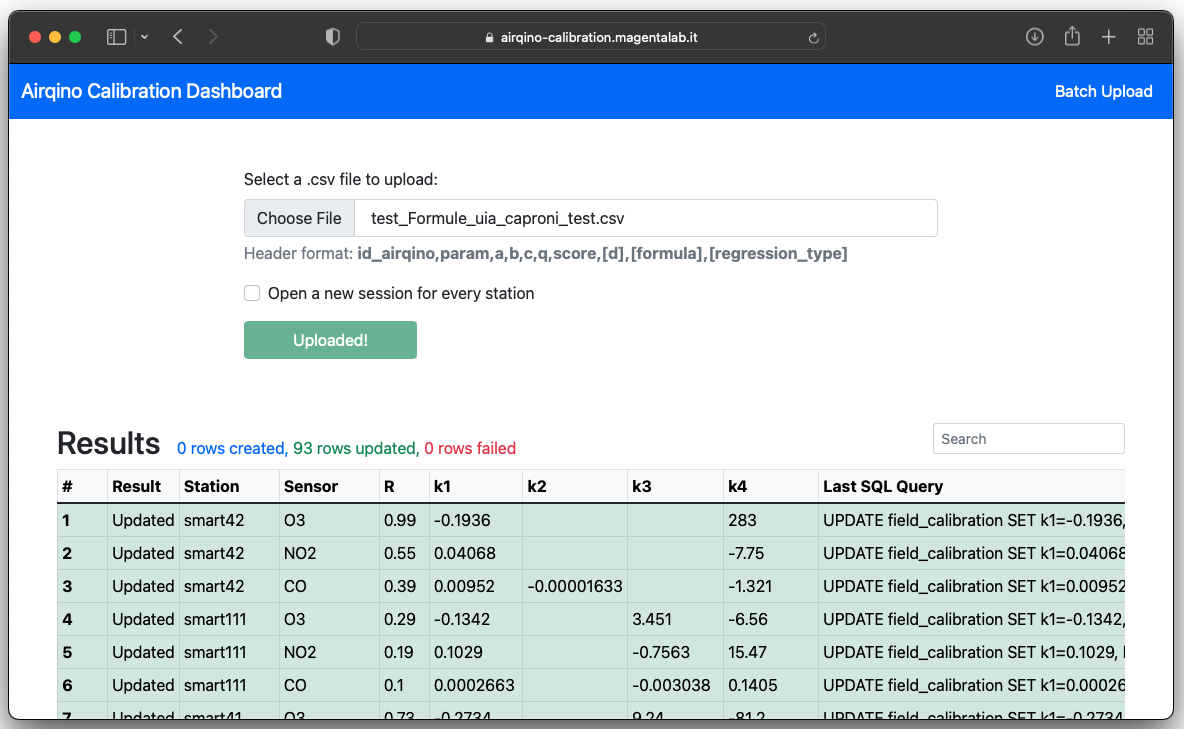
\includegraphics[width=\textwidth]{images/interfaccia_2_r}
\caption{Pagina web calibrazione}
\end{figure}
\end{center}

\end{column}

\end{columns}
\end{frame}

\begin{frame}{Interfaccia utente web (2/2)}
\begin{columns}

\begin{column}{0.43\textwidth}

\begin{itemize}
  \item Distinzione visiva per esiti diversi di ciascun sensore
  \item Con un meccanismo di \textbf{autenticazione} per proteggere da utenti di terze parti (\textit{Keycloak})
  \item Processo di rilascio automatizzato (\textit{CI/CD}) con isolamento delle dipendenze (\textit{Docker})
\end{itemize}

\end{column}

\begin{column}{0.65\textwidth}

\begin{center}
\begin{figure}[H]
\centering
\captionsetup{justification=centering}
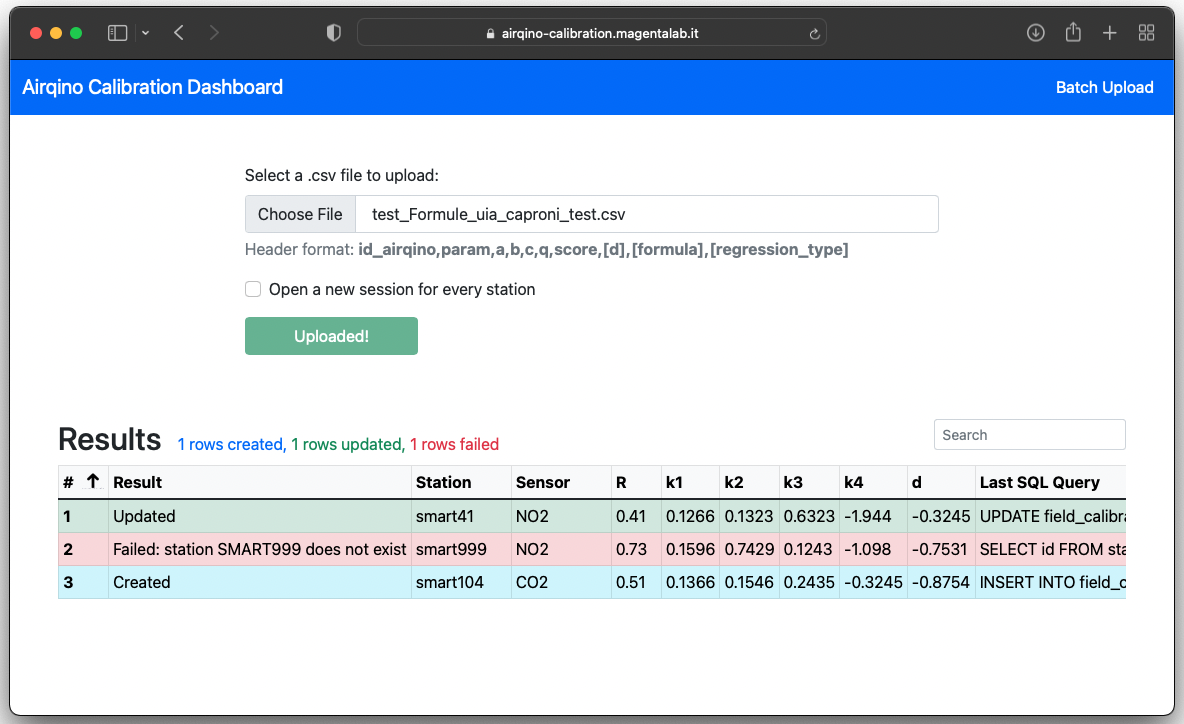
\includegraphics[width=\textwidth]{images/interfaccia_7}
\caption{Calibrazione con esiti diversi}
\end{figure}
\end{center}

\end{column}


\end{columns}
\end{frame}


\section{Conclusioni e sviluppi futuri}
\begin{frame}{Conclusioni e sviluppi futuri (1/2)}
\begin{itemize}
  \item Reti di sensori \textit{low-cost} per il monitoraggio della qualità dell'aria (es. \textbf{AirQino}) rappresentano una soluzione efficace per il rilevamento dell'inquinamento atmosferico\vspace{0.2cm}
  \begin{itemize}
    \item Anche in ottica di \textbf{integrazione} con le reti di monitoraggio regionali già esistenti, fornendo un quadro più completo della qualità dell'aria in ambiente urbano
  \end{itemize}\vspace{0.2cm}
  \item Anche con sensori a basso costo è possibile misurare inquinanti come \ce{NO2}, \ce{PM_{2.5}} e \ce{PM10}\vspace{0.2cm}
  \begin{itemize}
    \item Con accuratezza ancora migliore se si ha a disposizione un \textbf{segnale di riferimento} con cui correggere i dati provenienti dai sensori\vspace{0.1cm}
    \item L'applicazione di tecniche di \textbf{regressione robusta} in fase di calibrazione ha riportato miglioramenti significativi
  \end{itemize}
\end{itemize}
\end{frame}

\begin{frame}{Conclusioni e sviluppi futuri (2/2)}
\begin{itemize}
  \item Perfezionare il processo di calibrazione delle centraline, ad esempio implementando regressioni \textit{multivariate} (includendo fattori metereologici quali \textbf{temperatura} ed \textbf{umidità} relativa)\vspace{0.1cm}
  \begin{itemize}
    \item La \textbf{temperatura} tende a correlare negativamente con i PM (all'aumentare della temperatura le polveri sottili tendono a calare)
    \item L'\textbf{umidità} presenta l'effetto contrario e influisce anche sull'elettronica del sensore
  \end{itemize}\vspace{0.1cm}
  \item Realizzare una procedura di \textbf{anomaly detection} sul segnale delle centraline\vspace{0.1cm}
  \begin{itemize}
    \item Con un controllo \textbf{in tempo reale} sull'andamento e monitorando la differenza con il segnale di riferimento (es. stazione ARPAT)
    \item \textbf{Post processing analysis}
  \end{itemize}
\end{itemize}
\end{frame}

\begin{frame}[noframenumbering]{Grazie per l'attenzione!}
\begin{center}
\includegraphics[width=.9\textwidth]{images/airqino_web_n}
\end{center}
\end{frame}

